\documentclass[notitlepage]{report}
\usepackage[left=1in, right=1in, top=1in, bottom=1in]{geometry}

%Para usar colores en las tablas:
\usepackage{color}
%\usepackage{graphicx} DUPLICADO
\usepackage{epsfig}
\usepackage{multirow}
\usepackage{colortbl}
\usepackage[table]{xcolor}
%Fin de pacquetes para usar colores en las tablas


\usepackage{titling}
\usepackage{lipsum}
\usepackage{mathtools}
\usepackage{amsmath}
\usepackage{amsfonts}
\usepackage{amssymb}
\usepackage{pdfpages}
\usepackage[spanish]{babel}
\usepackage[utf8]{inputenc}
\setlength{\parskip}{2mm}
\usepackage{graphicx}
\graphicspath{ {../Imagenes/Editadas/} } 

%Definiendo colores:
\definecolor{lightgray}{gray}{0.9}
\definecolor{myblue}{RGB}{180,241,231}
\definecolor{myred}{RGB}{241,121,108}
\definecolor{myyellow}{RGB}{245,239,122}
%Fin de definicion de colores:


\pretitle{\begin{center}\Huge\bfseries}
	\posttitle{\par\end{center}\vskip 0.5em}
\preauthor{\begin{center}\Large\ttfamily}
	\postauthor{\end{center}}
\predate{\par\large\centering}
\postdate{\par}

\title{Diagonalización Inversa} 
\author{Juan Carlos Caso Alonso y Francisco Mario Cruz Almeida}
\date{\today}


\begin{document}
	
	\maketitle
	\thispagestyle{empty}
	
	\newpage
\renewcommand{\abstractname}{Abstract}
\begin{abstract}
	
	Testar la veracidad del Teorema de Cantor, no debería llevarnos a ningún lado excepto comprobar su solidez. Digamos que en el viaje realizado, buscando formas de ponerlo a prueba, me he encontrado una serie de fenómenos numéricos. 
	
	
	Algunos son solo redescubrimientos de cosas conocidas. Otros son cosas interesantes, aparentemente nuevas, pero sin demasiada relevancia en el campo de la teoría de conjuntos. Por ejemplo: haber encontrado un patrón común entre diversas biyecciones famosas, creando alternativas al uso de números primos.
	
	
	Pero hay dos fenómenos numéricos bastante curiosos. Por separado, sobre cada uno de ellos, han opinado dos matemáticos diferentes sin conocer la existencia del otro fenómeno. Lo curioso es que las contra-argumentaciones de ambos, se vuelven contradictorias, cuando mezclamos ambos fenómenos en uno: un intento de diagonalización inversa. La contra-argumentación de uno, le quita la razón al otro y viceversa.
	
	
	Un proceso, la diagonalización inversa, por el cual intentaremos 'afirmar' una consecuencia cardinal entre un conjunto, LCF, con el mismo cardinal que $\mathbb{N}$ y otro conjunto, SNEIs, con el mismo cardinal que $P(\mathbb{N})$. La novedad es que invertiremos los papeles: partiremos de afirmar que SNEIs tiene un cardinal mayor que LCF, y para que eso suceda, debe ser 'posible' hallar una 'muestra', muy concreta, de esa diferencia cardinal. La gracia va a estar en que nos va a resultar totalmente imposible hallarla. Y para 'mostrarlo', dada la singularidad del caso, podremos usar argumentos tremendamente similares a los de la diagonalización.
	
	
	Al final vamos a obtener un fenómeno con las mismas fortalezas y debilidades que dos técnicas de diagonalización usadas por Cantor. Y uso el término 'debilidades', pues las contra-argumentaciones a este fenómeno tienen 'traducción' directa en las diagonalizaciones cantorianas, donde no se consideran 'debilidades'. Las similitudes van a ser tremendamente asombrosas.
	
	
	Por eso, este documento consistirá en la exposición de varios fenómenos numéricos, y de explicar como funcionan en equipo para crear la susodicha diagonalización inversa.
	
	
	A pesar de usar definiciones correctas, siempre comienzan diciéndome que son confusas, para acabar aceptando su validez. Simplemente por su densidad inicial. No siendo, las definiciones, totalmente formales, se entienden rápida y perfectamente. No hay forma de acelerar o suavizar el viaje, así que tendremos que ir con calma, explicando y definiendo los conceptos del contexto de dichos fenómenos. Va a ser triste, por la simpleza de muchos de ellos... pero la experiencia me indica que es un viaje inevitable. Juro que las mismas personas han pasado de decir cosas como 'ininteligible' o 'confuso', a cosas como 'obvio' o 'trivial', simplemente por no haberlo leído bien, dado el tema que 'sobrevuela' a mi trabajo.
	
	
	Una vez expuestos, que cada cual les encuentre el sentido que desee. Pero su existencia es innegable.
			
\end{abstract}
		
	\addtocontents{toc}{\hspace{-7.5mm} \textbf{Capítulos}}
	\addtocontents{toc}{\hfill \textbf{P\'agina} \par}
	\addtocontents{toc}{\vspace{-2mm} \hspace{-7.5mm} \hrule \par}
	
	\tableofcontents
	
	\part{Parte I: Construcción de la diagonalización inversa}
	
	´\chapter{Introducción}

Vamos a intentar explicar a qué tipo de documento se enfrenta el lector.

Lo primero es aclarar que esto no es un paper. Por diversos motivos, como por ejemplo, no tener bibliografía. El motivo radica en que se me crea o no, muchas cosas son re-descubrimientos, y otras referencias me vienen por charlas informales con matemáticos, a lo largo de varios años.

Pero en realidad el formato concreto no debería ser importante si el contenido es interesante.

Tampoco va a tener el formato teorema-demostración, aunque al menos si van a haber muchas definiciones. Cuando enunciemos una propiedad, trataremos de explicar por qué funciona. Ya he comprobado que esto tampoco es ningún problema, pues quién ha puesto un poco de interés, acaba juzgando muchas de ellas como obvias y triviales. Incluso hay gente que llega a afirmar que es incapaz de señalar dónde está el fallo de las afirmaciones que hago.

El motivo de esta última versión es que SI hay dos personas que han encontrado dos, posibles, fallos diferentes. La gracia está en que sus contra-argumentaciones son contradictorias. El argumento de cada uno, convierte en importante el punto que desconoce, y sirve para negar la contra-argumentación del otro. Y juntando ambos puntos se produce un fenómeno que, espero, sea considerado como extremadamente interesante.

También la experiencia me dicta que muchos van a tratar de insistir en que cite el fallo de las demostraciones de los teoremas que son el origen de este trabajo. Los ejemplos más simples son solo una pérdida de tiempo, y resumir el fenómeno numérico que realmente los pone en jaque, a mi, me resulta imposible. Nada obliga a que un "error" sea sencillo de explicar o puntualizar. Si lo fuese, ya se hubiese descubierto hace tiempo.

Este documento tiene la intención de presentar dicho fenómeno numérico, y que el lector juzque sus consecuencias. El fenómeno es real, es "mostrable" y es "explicable" pues todas sus propiedades, aunque sean muchas, son "triviales" y "obvias". Y no lo digo yo... son palabras de otra gente extraídas a regañadientes. Muchas de las evidencias usadas son innegables. Pero para entender el fenómeno, hay que entender muchos conceptos del contexto que le dio vida.

El contexto del fenómeno numérico es un intento de rebatir el Teorema de Cantor mediante un contra-ejemplo. Ese es su contexto, no el objetivo, por obligación del rigor, de este documento. Deberemos estudiar todas las herramientas diseñadas a tal efecto... para llegados a un punto, construir y explicar el fenómeno numérico.

Cómo un ultimo intento de mejorar la experiencia lectora, producto de críticas previas, durante el escrito veremos las marcas:\\\\
\noindent<comentario complementario: <<Numero::indicación de tipo>> > \\\\
\noindent Se supone que dicho comentario contendrá material NO NECESARIAMENTE RIGUROSO, ya que no debería ser tenido en cuenta a la hora de juzgar este trabajo. Ejemplos, anécdotas, experiencias personales sobre ciertas contra-argumentaciones solventadas, orígenes de los conceptos, etc... Para poder leer cada uno, bastará con acudir al capítulo que recopilará dichos comentarios, y buscarlo indicado por su referencia numérica, como un sub-apartado de dicho capítulo.

Así se podrá elegir si tener o no, una experiencia lo más aséptica posible. También lo más rigurosa posible, dadas mis capacidades.

Otro problema al que nos enfrentaremos es que no se trata de un trabajo lineal... es más bien un árbol de ideas. Procuraré ceñirme al hilo argumental de crear el fenómeno numérico, y clasificar el resto como comentarios complementarios. Pero uno de los problemas, que ya he visto en el pasado, es que al no mencionar otras ramas, se piense que lo construido es el límite de lo que se puede lograr, que no se comprenda bien el verdadero potencial de las construcciones LJA, o que se sienta la tentación de usar ciertas contra-argumentaciones. También de que la "ausencia" de una rama, cree la tentación de afirmar que no existe.

Así que esto pretende ser una recopilación de todos mis escritos, con un proceso nuevo añadido, después de darme cuenta de las contradicciones en ciertas contra-argumentaciones.

El capítulo de las Construcciones LJA, probablemente se divida en dos: lo estrictamente necesario para crear el fenómeno numérico, que de por sí es largo, y otro capítulo, probablemente también complementario, expandiendo la técnica y mencionando técnicas más avanzadas.

En caso de que se considere el fenómeno numérico como digno de estudio o de gran valía para la comprensión de las cardinalidades infinitas, hay muchas ramas abiertas, y soluciones a medias, que dependen precisamente de ese juicio. Pero intentaré alejarlas de la rama principal, pues son dependientes del juicio de la comunidad matemática, aunque yo tenga mi propia opinión al respecto de su valía. Y serán mencionadas con la esperanza de que sirvan como pistas, para futuros posibles estudios que cuenten con los recursos adecuados.

Y como se dice en el abstract, el fenómeno numérico es una diagonalización inversa. Una construcción de diagonalización entre dos conjuntos, con cardinalidades iguales a $\mathbb{N}$ y $P(\mathbb{N})$, donde intercambian sus papeles tradicionales, generando propiedades tremendamente similares a las diagonalizaciones conocidas.

Mi esperanza es que la existencia de dicho fenómeno lleve a dos posibles conclusiones a todo aquel que tenga la paciencia para estudiarlo:

1) El argumento original es erróneo: con él, se puede demostrar lo mismo y lo contrario.

2) O la existencia de esta construcción demuestra que tienen el mismo cardinal.

Pero ese juicio no quiero afirmarlo, primero observadlo, y luego decidid por vosotros mismos. Aunque yo pueda estar equivocado con las consecuencias, algunas herramientas que uso presentan ciertas innovaciones. Menos espectaculares que la conclusión que yo deseo que se comparta, pero interesantes en si mismas.

Advierto, en mi intención de ser honesto, que uno de los puntos más débiles será la "solución multiverso"... que en realidad tiene "sentido cardinal", pero retuerce demasiado las definiciones. Os corresponderá juzgar si las he retorcido demasiado, o entra dentro de parámetros aceptables. Esto y juzgar las similitudes con las propiedades de las construcciones de diagonalización. El resto es tan sólido, que aún enunciado sin rigor, mucha gente se ve obligada a admitir su validez.

Y si un fenómeno, o un ejemplo concreto, lleva a plantearnos la validez de teoremas, o incluso axiomas... es independiente de la validez de su existencia. Ésta debe ser juzgada de forma independiente, siempre y cuando no viole ninguno de ellos, sino que muestre sus posibles contradicciones. 



	\input{CAPITULOS/CAPITULO_02/Chapter_02_Introduccion.tex}
	\chapter{Teorema CA}

\newpage
\section{Relaciones no aplicación}
Uno de las herramientas de este trabajo van a ser relaciones que no son aplicación: simples correspondencias. Y no serán 'función', porque por cada elemento del conjunto Dominio, a veces, tendremos relacionados más de un elemento del conjunto Imagen. Y no serán varios elementos dentro de un conjunto, sino que serán varios pares de la relación, cuyo elemento del Dominio es el mismo, pero cambian los elementos del conjunto Imagen, en cada par.

Por ejemplo:

\noindent Siendo el conjunto $X=\{a,b,c\}$ y el conjunto $Y=\{1,2,3,4,5,6,7,8,9\}$, y una relación $r:X \rightarrow Y$, los pares no serán del estilo:\\
$a \rightarrow \{1,2\}$, pues esto no sería una relación entre X e Y, sino entre X y un subconjunto de P(Y).\\\\
\noindent Sino que serán del estilo:\\
$a \rightarrow 1$\\
$a \rightarrow 2$\\\\
\noindent Formándose los pares (a,1) y (a,2)

No serán herramientas exclusivas, pues según el caso, usaremos inyecciones, biyecciones, o cualquier otra herramienta que nos permita obtener deducciones sobre los cardinales de los conjuntos envueltos. Siempre explicando el motivo por el cual nos permitimos la licencia de usar esa herramienta y no las conocidas. 

NO IMPORTA que las herramientas que usemos sean enrevesadas o poco elegantes, ni incluso que existan alternativas más sencillas... simplemente deben ser correctas y estar lo mejor definidas posible.

\newpage
\section{Concepto de Pack}
\noindent
Sea $f:X \rightarrow Y$\\ 
correspondencia entre conjuntos cualesquiera.\\

\noindent 
Sea $a \in X$ definimos:\\
$f(a) = \{ b \in Y / f(a) = b \}$\\ 
el conjunto imagen mediante la correspondencia $f$ del elemento $a$ de $X$.\\

\noindent 
Llamamos 'Pack' de $a$ a todo subconjunto NO VACÍO de $f(a)$.

\newpage
\section{Teorema CA}
 
Sean los conjuntos con cardinal transfinito cualesquiera:\\\\
$A = \{ a_{1}, a_{2}, ... , a_{n}, ... \}$\\
$B = \{ b_{1}, b_{2}, ... , b_{n}, ... \}$\\\\
Con $b_{i} = \{ c_{i1}, c_{i2}, ..., c_{ir}, ... \}$ \\\\
Siendo \textbf{todos} los $b_{i}$ disjuntos entre sí.\\

Hacemos la biyección de A en B tal que:\\\\
$f: A \rightarrow B$\\
$\:\:a_{i} \rightarrow f(a_{i})=b_{i}$\\

Es evidente que es una biyección.\\

Está \textbf{bien definida}:\\
$\forall a_{i} \in A$,  $\exists f(a_{i}) = b_{i} \in B$

Es \textbf{aplicación}:\\
Si $a_{i}=a_{j} \:\:\:\Rightarrow\:\:\: i=j$\\
Y esto implicaría\\
$f(a_{i}) = b_{i} = b_{j} = f(a_{j})$\\
Por lo tanto es aplicación.

Es \textbf{inyectiva}:\\
Si $f(a_{i}) = f(a_{j}) \:\:\:\Rightarrow\:\:\: b_{i}=b_{j}$\\
Como los Packs son disjuntos $\Rightarrow i=j \:\:\:\Rightarrow\:\:\:a_{i}=a_{j}$

Es \textbf{sobreyectiva}:\\
$\forall b_{i} \in B: \: b_{i} = \{c_{i1}, c_{i2}, ... , c_{ir}, ... \}$\\
$\exists a_{i}: \: f(a_{i}) = b_{i}$\\
Por lo tanto es biyectiva.

Como $f(a_{i}) = b_{i} = \{c_{i1}, c_{i2}, ... , c_{ir}, ... \}$. Entonces $|A| \ngtr |B|$, aunque no sea biyección.
\newpage
Por ejemplo, si con la misma relación:
\begin{figure}[h!]
	%width=\textwidth
	%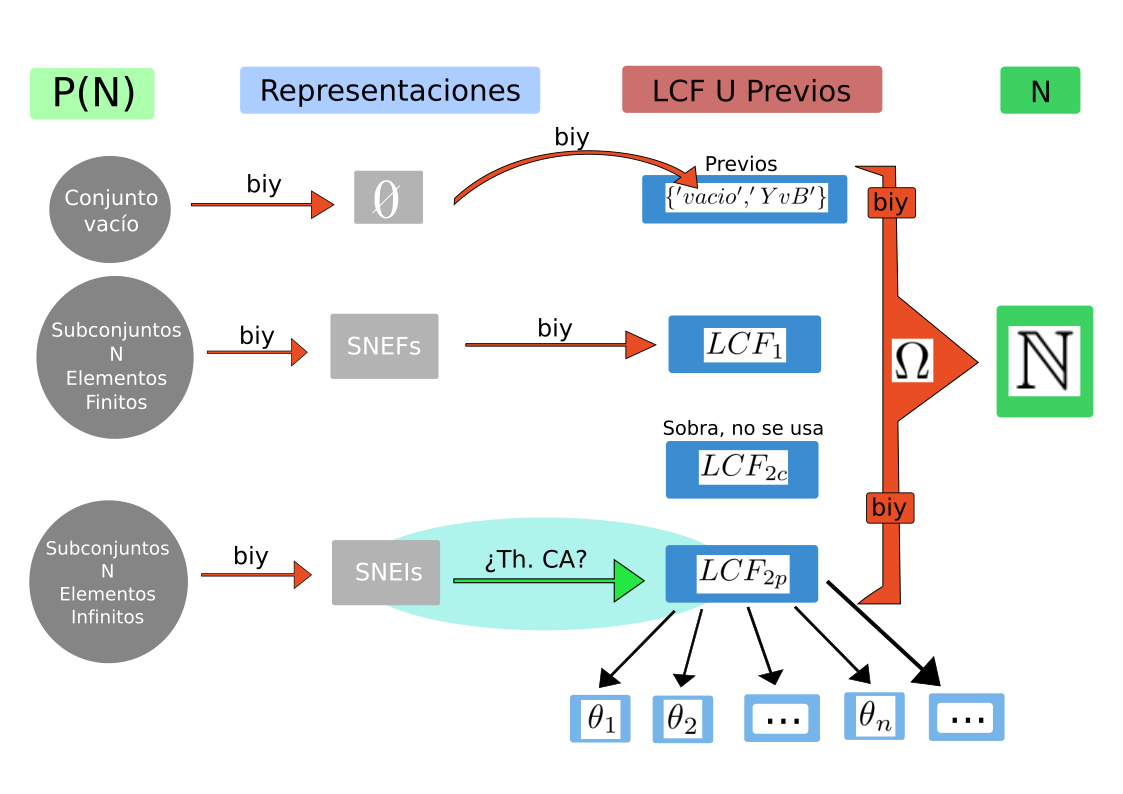
\includegraphics[ scale=0.7, angle=90]{EsquemaRelaciones}%
	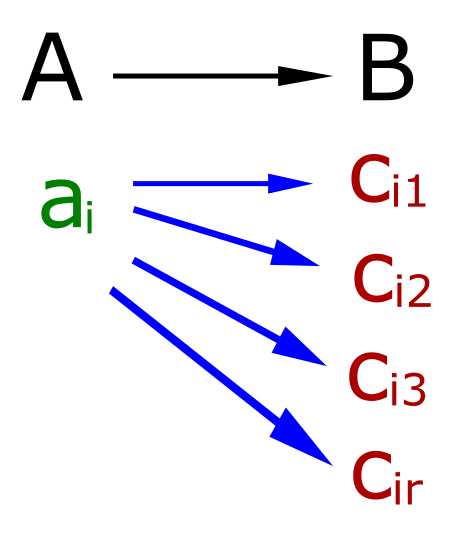
\includegraphics[scale=0.5]{cap02/ImagenNoAplicacion}
	%\includegraphics[width=\textwidth, scale=0.3]{Funcion_hx_002_v4}
	%\includegraphics[width=\textwidth, scale=0.3]{Funcion_hx_001_v4}
	\centering
\end{figure}\\
%\noindent%
%$i \in I=\{ 1, 2, ..., r, ...\}$\\%

En este caso partimos de una simple correspondencia, pues desde que $r\geq 2$ no sería aplicación. Pero tendríamos que $|A| \ngtr |B|$ pues de cada $a_{i}$ sale al menos una flecha, por tanto el número de elementos de $B$ es, al menos, el mismo que el de $A$. Recordemos la regla que obliga a todos los $b_{i}$, a ser todos disjuntos entre sí.



%\newpage%
\section{Interpretación intuitiva}
Un buen ejemplo sería un cine infinito, con sus clientes, o un gallinero infinito con gallinas mutantes que han puesto infinitos huevos.

En el ejemplo del cine con butacas y clientes infinitos, nos daría igual el cardinal de cada conjunto. Simplemente sabiendo, que cada uno, de todos los posibles clientes, tiene tres butacas para su uso absolutamente exclusivo, podríamos afirmar que el cardinal del conjunto de clientes, no es mayor, que el cardinal del conjunto de las butacas. Daría igual si fuesen 3, 4, o infinitas butacas de uso exclusivo.

En el caso del gallinero, partimos de un gallinero infinito, con infinitas gallinas mutantes, que la noche anterior pusieron infinitos huevos. Sabemos con absoluta seguridad que todos los huevos tienen dos yemas cada uno. Ese es el poder de nuestras gallinas mutantes. Por lo tanto, podemos afirmar con total tranquilidad, que el cardinal del conjunto de los huevos puestos ese día, no es mayor, que el cardinal de las yemas, de los huevos puestos ese mismo día.

En ninguno de los dos casos, necesitamos preguntarnos que cardinal transfinito tiene cada conjunto.\\

\textbf{Partiendo de una relación no aplicación, entre los conjuntos $A$ y $B$:\\
1) Si para todo elemento de $A$, tenemos un Pack de elementos del conjunto $B$.\\
2) Y TODOS los Packs son no vacíos y disjuntos entre sí.\\
$\Rightarrow |A| \ngtr |B|$ }



$\langle$Comentario Complementario: $\langle\langle$1:Lo que pretendo que se deduzca$\rangle\rangle$

\newpage
\section{Equivalencias con el concepto de inyección}

El Teorema CA, ha acabado siendo una generalización no intencionada de la función inyectiva. Igualmente lo usamos para poder afirmar que el cardinal de un conjunto, no es mayor que el cardinal de otro conjunto. La inyectividad, es un caso particular del teorema.

Pero ahí se acaban las similitudes... Sería un error estar buscando constantemente la alternativa inyectiva de las relaciones que usemos. Lo que buscaremos será abusar y retorcer, las capacidades de las propiedades de los Packs con cardinal transfinito.

Hasta tal punto, que dónde matemáticamente fracasan los conceptos de inyectividad o biyectividad, los Packs transfinitos generarán fenómenos numéricos innegables. Fenómenos que espero generen muchas dudas como mínimo.
	
	\part{Parte II: Anexo de comentarios complementarios}
	
	\chapter[Ordenados por referencias, no por aparición]{Comentarios Complementarios}

\section {Lo que pretendo que se deduzca:}

\noindent 1) Cuando todos los Packs que escogemos, de la relación, tienen cardinal uno, es un caso de equivalencia total con una función inyectiva.\\\\
\noindent 2) Los Packs pueden tener cardinales diferentes, y aún así respetarse las condiciones para que se cumpla el Teorema CA.\\\\
\noindent 3) Los Packs pueden tener cardinalidad transfinita.\\\\

En su día partimos de la sospecha que la diferencia entre $\mathbb{R}$ y $\mathbb{N}$ era los Irracionales. Que los números Irracionales formasen cadenas infinitas de símbolos era lo que provocaba que no se pudiesen encontrar biyecciones entre ambos conjuntos. Su diferencia no era realmente cardinal. Con eso en mente, y gracias a las estructuras que se pueden construir con las CLJAs, decidimos asignar un natural diferente a cada 'símbolo' del número Irracional. Si realmente eran únicos, alguna parte de su cadena debía ser única y diferente a la del resto de números Irracionales... y como había un natural por cada símbolo... en esa parte única tendríamos, una serie de naturales únicos, asignados a cada número Irracional.

De ahí que los Packs que usemos tengan cardinal transfinito. Cuando veamos la definición de la correspondencia flja\_abstracta, junto con la biyección $\Omega$ (La función flja de la Clja\_FTC), veremos como cada natural está asociado a cada 'etiqueta' de un SNEI (en cada universo). Incluso como la misma etiqueta, en la misma posición, recibe un natural diferente pq depende del resto de etiquetas anteriores. Sucederá que, ante la primera diferencia de etiquetas, aunque el resto sean idénticas en las mismas posiciones, la serie de números naturales asignados comenzará a ser diferente. A ser 'disjuntos'.

La responsable de esta propiedad será la CLJA, que tiene muchas similitudes con un grafo tipo árbol. Aunque dos nodos, tengan el mismo nombre, pero estén en diferentes ramas, en realidad serán nodos diferentes. Y una de las propiedades de la CLJA es poder asignar un natural único a cada uno de sus 'huecos azules' (el concepto equivalente a nodo).

Pero la distribución que genera es TAN caótica... aparte de no tener sentido lexicográfico, ha creado la necesidad del concepto de Pack, y de los universos, por un simple potencial que se descontrola muy fácilmente. Para crear biyecciones hay que afinar muchísimo o generas aberraciones combinatorias. O correspondencias que crean las condiciones para que podamos aplicar el Th CA. O ambas a la vez en un caos maravilloso. Entre los SNEFs y $LCF_{1}$, hay una biyección. Entre los SNEIs y $LCF_{2}$, hay una correspondencia... sobre la que estudiaremos si podía o no cumplir el Th CA. Pero todo parte de la misma CLJA.   

\newpage

\section {2: Segundo comentario}

Segundo comentario :D.

\newpage
	
\end{document}